\documentclass[sigconf,review,anonymous]{acmart}
\settopmatter{printfolios=false,printccs=false,printacmref=false}

\AtBeginDocument{%
  \providecommand\BibTeX{{%
    \normalfont B\kern-0.5em{\scshape i\kern-0.25em b}\kern-0.8em\TeX}}}

\setcopyright{none}
\copyrightyear{2018}
\acmYear{2018}
\acmDOI{10.1145/1122445.1122456}

\acmConference[ICSE 2022]{The 44th International Conference on Software
Engineering}{May 21–29, 2022}{Pittsburgh, PA, USA}

\usepackage{algorithmic,xspace,graphicx}
\usepackage{xcolor,listings,listings-djanco,rotating}
\usepackage{hyperref}

% Kable includes (latex table from Rmds)
\usepackage{booktabs,enumitem,multirow}
\usepackage{longtable}
\usepackage{array}
\usepackage{float}
\usepackage{colortbl}
\usepackage{pdflscape}
\usepackage{tabu}
\usepackage{threeparttable}
\usepackage{threeparttablex}
\usepackage[normalem]{ulem}
\usepackage[utf8]{inputenc}
\usepackage{makecell}
\usepackage{xcolor}
\usepackage{tikz}
\usepackage{caption}
\usepackage{subcaption}

\newcommand{\gh}{{GitHub}\xspace}
\newcommand{\git}{\texttt{git}\xspace}
\newcommand{\ght}{{GHTorrent}\xspace}
\renewcommand{\dj}{{\textsf{Code{\small{DJ}}}}\xspace}
\newcommand{\para}{\textsf{Parasite}\xspace}
\newcommand{\djco}{\textsf{Djanco}\xspace}
% todo change these to ticks/emojis/whatever
\newcommand{\yes}{{Y}}
\newcommand{\no}{{--}}
\newcommand{\abit}{{b}}
\newcommand{\rot}[1]{\begin{sideways}#1\end{sideways}}
\newcommand{\eg}{e.g.\xspace}
\usepackage{../latex-include/dataset}
\usepackage{../latex-include/scent_dl}
\usepackage{../latex-include/method_chaining}
\usepackage{../latex-include/style_analyzer}
\usepackage{../latex-include/software}

\begin{document}
\title{The Fault in Our Stars}
\subtitle{How to Design Reproducible Large-scale Code Analysis Experiments}

\lstset{
  language=dejaco,
  style=dejaco,
  frame=none,
  lineskip=-.6pt,
  aboveskip={1.5mm},
  belowskip={1mm},
  }
\renewcommand{\c}[1]{\lstinline|#1|\xspace}

\begin{abstract}
  Software engineering benefits from the insights gleaned from large-scale
  software repositories as they offer an unmatched window into the software
  development process. Their sheer size holds the promise of broadly applicable
  results. At the same time, that very size presents scalability challenges. The
  traditional answer to such challenges is to limit studies to representative
  samples and generalize observations to the entire population. The contribution
  of this paper is both modest and, we believe, important. We advocate in favor
  of a standardized experimental design methodology for experiments over large-scale
  repositories. In particular, we steer researchers away from using extrinsic
  attributes such as stars, and emphasize careful delineation of the population
  of interest backed up by random sampling of inputs.
\end{abstract}
%\ccsdesc[500]{ Software and its engineering → Ultra-large-scale systems;}
%\keywords{software, mining code repositories, source code analysis}
\maketitle

\section{Introduction}

And so it begins

\begin{quote}\small\it
We count the number of stars associated with each repository. The number of
stars relate to how many people are interested in that project. Thus, we assume
that stars indicate the popularity of a project. We select the top 50 projects
in each language...
\end{quote}

\noindent
Sentences like these appear in the methodology sections of our papers. They are
often all there is to be found in terms of experimental design. This paper aims
to convince readers of the dangers that this state of affairs presents for
generalizability and reproducibility of our results and to suggest some simple
improvements.

Large-scale code repositories such as \gh are a boon to the software
engineering community as they give us a large body of software along with
metadata written in many languages with various degrees of care and expertise.
The number of artifacts for each of the major language ecosystems ranges in the
millions. With a little patience and enough storage, a researcher can acquire
thousands of projects for their latest research effort. Unfortunately, obtaining
an entire ecosystem is difficult, and analyzing it may be prohibitive -- in
hardware resources and researcher effort.

Empirical software engineering studies are experiments performed on a corpus of
software to validate some hypothesis. The value of any given experiment does not
lie in what learn about the projects that were analyzed, but rather in what they
teach us about the larger population. There is little value in, say, learning
that 10 particular Java projects adopted a new language feature if we cannot
generalize that result to a broader portion of the ecosystem. Yet, few papers
articulate their claims of generality and it is often not even clear how
researchers selected the software artifacts they studied.

Table~\ref{tbl:msr-summary} has a meta-study of two editions of \emph{Mining
Software Repositories} (2019, 47 papers; 2020, 45 papers). Out of 92 papers, 29
do not have an experimental component that involves software, 16 analyze very
small curated datasets, and 18 use the entire available populations. This leaves
29 papers which analyze code obtained from a larger population: 4 are not
reproducible, lacking information about how their dataset was constructed or
using proprietary data, 14 use \gh stars to filter projects, 6 use
combinations of attribute thresholds and only 5 use random sampling. In
summary, out of 29 large-scale code analysis papers, 48\% rely on stars.

\begin{table}[!h]
\begin{tabular}{@{}r@{~} c cl@{}}\toprule
\bf papers&\bf projects&\bf classification&\bf description\\\midrule\midrule%}
 29 & --       & incompatible & No experiments\\
 16 & --       & curated      & Small curated datasets \\
 18 & --       & everything   & Entire population\\\midrule
  4 & 1--35K   & unknown      & Unknown or proprietary\\
 14 & 5--2M    & stars        & Filter projects using stars \\
  6 & 7--290K  & other        & Other filter for projects \\
  5 & 6--51K   & random       & Filter and sample randomly\\
 \bottomrule
\end{tabular}
\caption{Experimental design summary (MSR 2019 and 2020)}\label{tbl:msr-summary}
\end{table}

\vspace{-2mm}

\noindent
Why do \gh stars play such a central role in our experimental methodology? We
want to think it is neither malice nor sloth, but rather expectations and
pragmatics. Community standards are set by the papers we publish. The literature
codifies expectations for authors of the next batch of papers. These
expectations slowly evolve in response to reviewer attitudes. So we use stars
because our peers do, but the pragmatics are just as important. \gh does not
provide an index of its projects, nor does it allow to query over intrinsic
attributes of code. Finding inputs is thus hobbled by limitations of our tools.
One wants to find projects of interest while avoiding the duplicates that litter
most language ecosystems and weeding out obviously uninteresting projects.
Absent any other tools, stars play a double role. First, they are an index of
projects, one that can be queried from the \gh interface. Second, there is an
expectation that they correlate with some notion of quality.
%%
But, not only do stars not accomplish that, they introduce reproduction barriers
into project selection. So what to do?

We propose a methodology for designing reproducible experiments with the
explicit goal of improving the generalizability of our results. The
methodology is in line with evolving community standards~\cite{Ralph:2021} but
specific to large-scale code analysis, and we emphasize the needed for proper
tooling to ensure reproducibility. Our approach takes the form of the following
protocol:

\begin{enumerate}[leftmargin=*]
\item {\bf Population Hypothesis:} A brief description of the population of
  interest, what the research should generalize to, which may be a narrow slice
  such as ``programs written by students learning JavaScript as their first
  language'' or a broader one such as ``commercial code''.
\item {\bf Frame Oracle:} A procedure for deciding if a project belongs to the
  population. Ideally, an algorithm efficiently computed over intrinsic
  attributes of a project. An oracle could, e.g., return \gh projects with one
  JavaScript file which were created by a user with no previous commits.
\item {\bf Sampling Strategy:} A strategy for selecting a subset of the values
  of the population. Ideally, specified algorithmically. An example is random
  sampling without replacement from a known seed.
\item {\bf Validity:} An argument about the oracle's and sampling strategy's
  validity as means to obtain representative samples from the population. A
  discussion of attempts to validate result quality, such as manual inspection
  of a sample to check if JavaScript code was actually written by beginners.
\item {\bf Reproduction Artifacts:} The artifact should allow to reproduce
  exactly the reported results as well as to change either the input or the
  experiment.
\end{enumerate}

\noindent
Reproducibility has nuances. We specifically do not talk about the experiment
itself -- others have been there before us. Instead our emphasis is on inputs
and support for the following three use cases: \emph{Repetitions} which run the
reproduction artifact to obtain bit-for-bit equal results (or as close as
feasible). This is the most stringent use case and often requires a reproduction
artifact that bundles code and inputs. \emph{Reanalysis} alters either the
method or its input, it requires an executable artifact and a method for
acquiring new inputs. Finally, \emph{reproductions} are independent
implementations that require the paper to have an unambiguous description of all
experimental details.

Design experiments that support reproducibility can be greatly simplified with
appropriate tooling. Our work builds on the open source \dj
infrastructure.\footnote{\url{https://codedj-prg.github.io}} Our contributions,
briefly, are:
\begin{enumerate}[leftmargin=*]
\item {\bf A dataset} of 2Mio+ Java, Python and JavaScript projects. Modified
  \dj to compute 36 intrinsic project attributes. (Sec.~4)
\item {\bf A characterization of stars} as a means to select inputs for code
  analysis experiments. (Sec.~4)
\item {\bf A methodology} that can be readily adopted by researchers to improve
  reproducibility of their work. (Sec.~5)
\item {\bf A reproduction} of four papers that highlights challenges to
  generality. (Sec.~3 and 6)
\end{enumerate}

\noindent
Our work is open source and reproducible.\footnote{A polished artifact will be
submitted for evaluation should our paper be accepted. For now, we share an
anonymized code bundle. We have several terabytes of data, the Program Chairs
kindly agree to act as intermediary should reviewers require access:
\url{https://github.com/unknown-john/ICSE21-Anonymized}}

\section{Related Work}

We review relevant advice, warnings and the state of tooling.

\newcommand{\mypara}[1]{\vspace{2mm}\noindent{\bf #1}~~}

%% https://github.com/acmsigsoft/EmpiricalStandards/blob/master/Supplements/Sampling.md

\mypara{Community Standards.} A strong push towards reproducibility is underway,
efforts such as the standards framework of \citet{Ralph:2021} include a section
on experimental design and specifically sampling. These ideas are further
explored by \citet{baltes20} who argue that software engineering faces a
generalizability crisis. They carried out a meta-analysis of 120 papers in all
areas of the field and report that purposive and convenience sampling are widely
used. Such sampling techniques rarely lead to representative samples, and --
without a careful study of potential sources of bias -- can lead to conclusions
that do not generalize. They explain this state of affairs by a fundamental
challenge in the field, the lack of appropriate sampling frames to access
elements of the population of interest. Earlier work by \citet{Nagappan:2013}
already attempted to address this problem by defining the notion of sample
coverage to assess the quality of the data used as input to an experiment. Even
closer to our paper is the study by \citet{Cosentino:MSR16} which reported that
out of 93 large corpus papers, 63 papers failed to provide replication datasets.
Most papers did not use random samples and omitted mentions of limitations.


\mypara{Mining Repositories.} \gh is extremely popular data source. Warnings
about perils go back to the work of \citet{Kalliamvakou:2014} who highlighted
``noise'' among hosted projects. In particular they point out that tiny and
inactive projects dominate the platform. \citet{oopsla17a} pour oil on that fire
by showing that up 95\% of the code in some language ecosystems were copies.
Stars are known to be widely used as a mean to find signal in that sea of noise.
But what do they mean? \citet{Borges:2018:JSS} surveyed users and found that the
most common reasons for starring a project are to show appreciation (e.g. {\it I
  starred this repository because it looks nice.}) and bookmark it (e.g. {\it I
  starred it because I wanted to try using it later.}). They also warn against
promotional campaigns in social media driving up ratings. Popularity of projects
was studied by \citet{Han:2019:COMPSAC} who suggest that while most users
believe stars are the best metric to determine popularity of a project, other
attributes such as branches, open issues and contributors are better predictors.
Expending on that result, \citet{mun17} propose to use random forest to create
a classifier for \emph{engineered projects}, which they define as projects that
leverage sound software engineering principles. Their classifier outperforms
stars. \citet{pick19} further improved classification with an approach based on
time-series clustering.

\mypara{Tools for Miners.} A number of infrastructures have been developed to
assist researchers in the field. The most ubiquitous is
\ght~\cite{Gousios:2012}, a continuously updated database of metadata about
public projects that is a valuable building block for other tools. Boa is
complementary as it lets users write sophisticated queries over source
code~\cite{Boa:2013}. \dj is a newer infrastructure that supports queries over
both meta-data and file contents~\cite{ecoop21}. Unlike Boa it is language
agnostic. \citet{ma21} and \citet{Mattis:2020:ACM} address performance issues of
querying at scale. Of these, only \dj ensures reproducible queries.

\section{State of Practice}

%What is the state of the art in experimental design
How do people design experiments for large-scale code studies? This section give
examples from the meta-study of Table~\ref{tbl:msr-summary}. We emphasize to the
reader, it is not our goal to criticize individual authors, but it is helpful to
establish a baseline to improve community best practices. Following our proposed
methodology, for each paper, we give a brief summary of the scientific claim
followed by an account of the paper's stated population hypothesis, a
description of the frame oracle, sampling strategy, validation and reproduction
artifacts. We conclude with some observations.

\renewcommand{\P}[1]{\vspace{1mm}\noindent{\it\underline{#1}}~~}

\newpage

\subsection{MSR 2020: What is Software}

``Software'' has an intuitive definition, namely code, but there is more.
\citet{Pfeiffer20} classifies the content of repositories in categories such as
code, data and documentation. They then observe that software is more than just
code. Documentation is an integral constituent of software, and software without
data is often correlated with libraries, and finally that software without code
is rare, but exists.

\P{Population Hypothesis:} The paper answers the question {\it ``what are the
  constituents of software and how are they distributed?''\,} The authors claim
that existing definitions of the term are non-descriptive, inconclusive and even
contradictory. Implicitly the population is all inclusive.

\P{Frame Oracle:} Any software project hosted on \gh.

\P{Sampling Strategy:} Convenience sampling; the authors chose popular
repositories and further clarify that {\it ``by popularity we mean the starred
  criteria with which \gh users express liking similar to likes in social
  networks.''\,}

Most-starred projects in 25 languages were acquired by executing one query by
language, saying that {\it ``without language qualifier, the API returns only
  1,020 repositories in total, which we decided is not enough for our study.''}

\P{Validity:} No discussion of relevant issues.

\P{Reproducibility Artifacts:} A listing of files and repositories is provided
with the code of the classifier. Figures and numbers produced by a notebook are also
included. The contents of the repositories analyzed are not preserved.

\subsection{MSR 2020: Method Chaining}

In an object-oriented language, a \emph{method chain} occurs when the result of
a method invocation is the receiver of a subsequent method call. In Java, method
chaining manifests as a sequence of calls connected by dots.
\citet{nakamaru:2020:MSR} analyze trends in usage of method chains and conclude
that their use increased over a period of eight years.

\P{Population Hypothesis:} Java projects developed {\it ``by real-world
  programmers.''\,} The authors state that they {\it ''did not apply any filter to
  the collected repositories. This supports the generalizability of our
  results.''}
The authors consider generalization beyond Java, saying {\it ``our
  results are more likely to be applied to a language that does not provide such
  a construct (e.g. PHP and JavaScript). The empirical study of this hypothesis
  is future work.''\,} The construct in question is support for DSLs.

\P{Frame Oracle:} Implicitly defined as all Java projects hosted on \gh.

\P{Sampling Strategy:} The authors use convenience sampling, taking 2,814
projects that appeared at least once in the list of the 1K most-starred projects
between November and December 2019. Projects were deduplicated and filtered for
syntactically invalid files.

\P{Validity:} --

\P{Reproducibility Artifacts:} Project metadata and computed chain len\-gths are
published.\footnote{https://zenodo.org/record/3697939\#.YSYcZ9OA63I}
Communication with the authors reveals that their complete reproduction package
is currently not available.

\subsection{MSR 2019: Style analyzer}

Each software project seems to develop its own formatting conventions.
\citet{Markovtsev:2019:MSR} demonstrate that an unsupervised learning algorithm
can automate project-specific code formatting. They reproduce the style of a
project with a high degree of precision on a dataset of repositories with one
base and one head commit specified for each.

\P{Population Hypothesis:} From statements made about the outcome of the
experiment, we surmise that the population is that of {\it ``real projects.''\,}
From tools, mechanics and the sample prepared for the experiment, we suppose the
authors aimed for developed projects. The population is implicitly limited to
JavaScript as the tool includes a parser for that language.

\P{Frame Oracle:} The oracle is implicitly all JavaScript project hosted on \gh.

\P{Sampling Strategy:} Convenience sampling: 19 JavaScript projects with high
numbers of stars are picked. Date of selection is not provided.

\P{Validity:} Authors manually inspected projects in the selection.

\P{Reproducibility Artifacts:} A \gh repository containing the tool and a file
with project URLs along with their head and base commits is
provided.\footnote{\url{https://github.com/src-d/style-analyzer}} Contents of
repositories are not included. Documentation, run scripts and configuration
information are patchy.

\subsection{MSR 2020: Code Smells}

Code smells are programming idioms that are often correlated with correctness or
maintenance issues. \citet{Jebnoun:2020:MSR} contrast code smells in projects
related to deep learning and general purpose software projects. Their scientific
claim is that for large and small projects there is a statistical difference in
the occurrence of code smells, whereas medium sized projects are
indistinguishable.

\P{Population Hypothesis:} The authors are interested in two populations: On one
hand projects that implement or use deep learning algorithms, and general
purpose software on the other. For pragmatic reasons, they focus on the Python
ecosystem as it is widely used for machine learning.

\P{Frame Oracle:} Projects must be in Python and hosted on \gh. Keyword
search is used for machine learning frameworks and technologies such Tensorflow and
Keras, discarding tutorials. Furthermore, the authors \textit{``also carefully select
  popular and mature DL projects from them by employing maturity and popularity
  metrics (e.g., issue count, commit count, contributor count, fork count,
  stars).''}

\P{Sampling Strategy:} A staged strategy was employed to sample both
populations. The authors relied on judgment sampling to manually select 59 deep
learning projects. For general purpose projects, they used a top-starred list of
106 Python projects from \citet{Chen:2018:IST} and randomly sampled 59 projects.
Projects were further clustered into small ($\leq\dlSlocSmall$), medium, and
large ($\geq\dlSlocMedium$).

\P{Validity:} --

\P{Reproducibility Artifacts:}  A listing of the 59 deep learning projects is
provided.\footnote{https://github.com/Hadhemii/DLCodeSmells/blob/master/data/dlRepos.csv}
%{\bf PETA Isn't there more? Like how they analyze the code smells? }

\newpage
\subsection{Reproducibility issues}

While these four research projects were done with care, none can be fully reproduced.
Reproducibility failures have many reasons, most of which are common to several
of the papers we have reviewed:
\begin{itemize}[leftmargin=*]
\item {\it Missing descriptions:} Failure to specify either one of: population
  hypothesis, frame oracle or sampling strategy. Reproduction is fraught with
  perils and an apple-to-apple comparisons between papers is difficult. This
  affects
  \cite{Pfeiffer20,nakamaru:2020:MSR,Markovtsev:2019:MSR,Jebnoun:2020:MSR} as
  their descriptions are open to interpretation.
\item {\it Missing projects:} Even with a list of URLs, the corresponding
  projects may vanish at any time (e.g., deleted or made private). Reproductions
  are partial at best, we have seen a project disappear while being
  downloaded. This affects
  \cite{Pfeiffer20,nakamaru:2020:MSR,Markovtsev:2019:MSR,Jebnoun:2020:MSR}.
\item {\it Fading stars:} Stars are volatile. \citet{nakamaru:2020:MSR} observed
  close to 3,000 projects in the top 1K during a period of two months. Without a
  history of star attribution and a timestamp, reconstructing the star
  listings is not possible. This affects \cite{Jebnoun:2020:MSR}.
\item {\it Shifting contents:} The contents of a project change with new
  commits. To reconstruct the data, ids of the last observed commit must be
  specified. Even that is not foolproof as Git histories can be updated
  destructively. This affects
  \cite{Pfeiffer20,nakamaru:2020:MSR,Jebnoun:2020:MSR}.
\item {\it Language attribution:} Projects contain code in many languages. For
  reproduction attribution must specified. While dlegating to, e.g. \gh, is
  reasonable, one should be aware that \gh has changed their attribution
  algorithm several times. Double counting a project is sometimes valid. This
  affects \cite{Pfeiffer20, nakamaru:2020:MSR,Markovtsev:2019:MSR}.
\item {\it Deterministic replay:} Non-determinism must be limited. Random
  sampling seeds should be specified. This affects
  \cite{Markovtsev:2019:MSR}.
\end{itemize}

\noindent

\begin{figure*}[!t]
    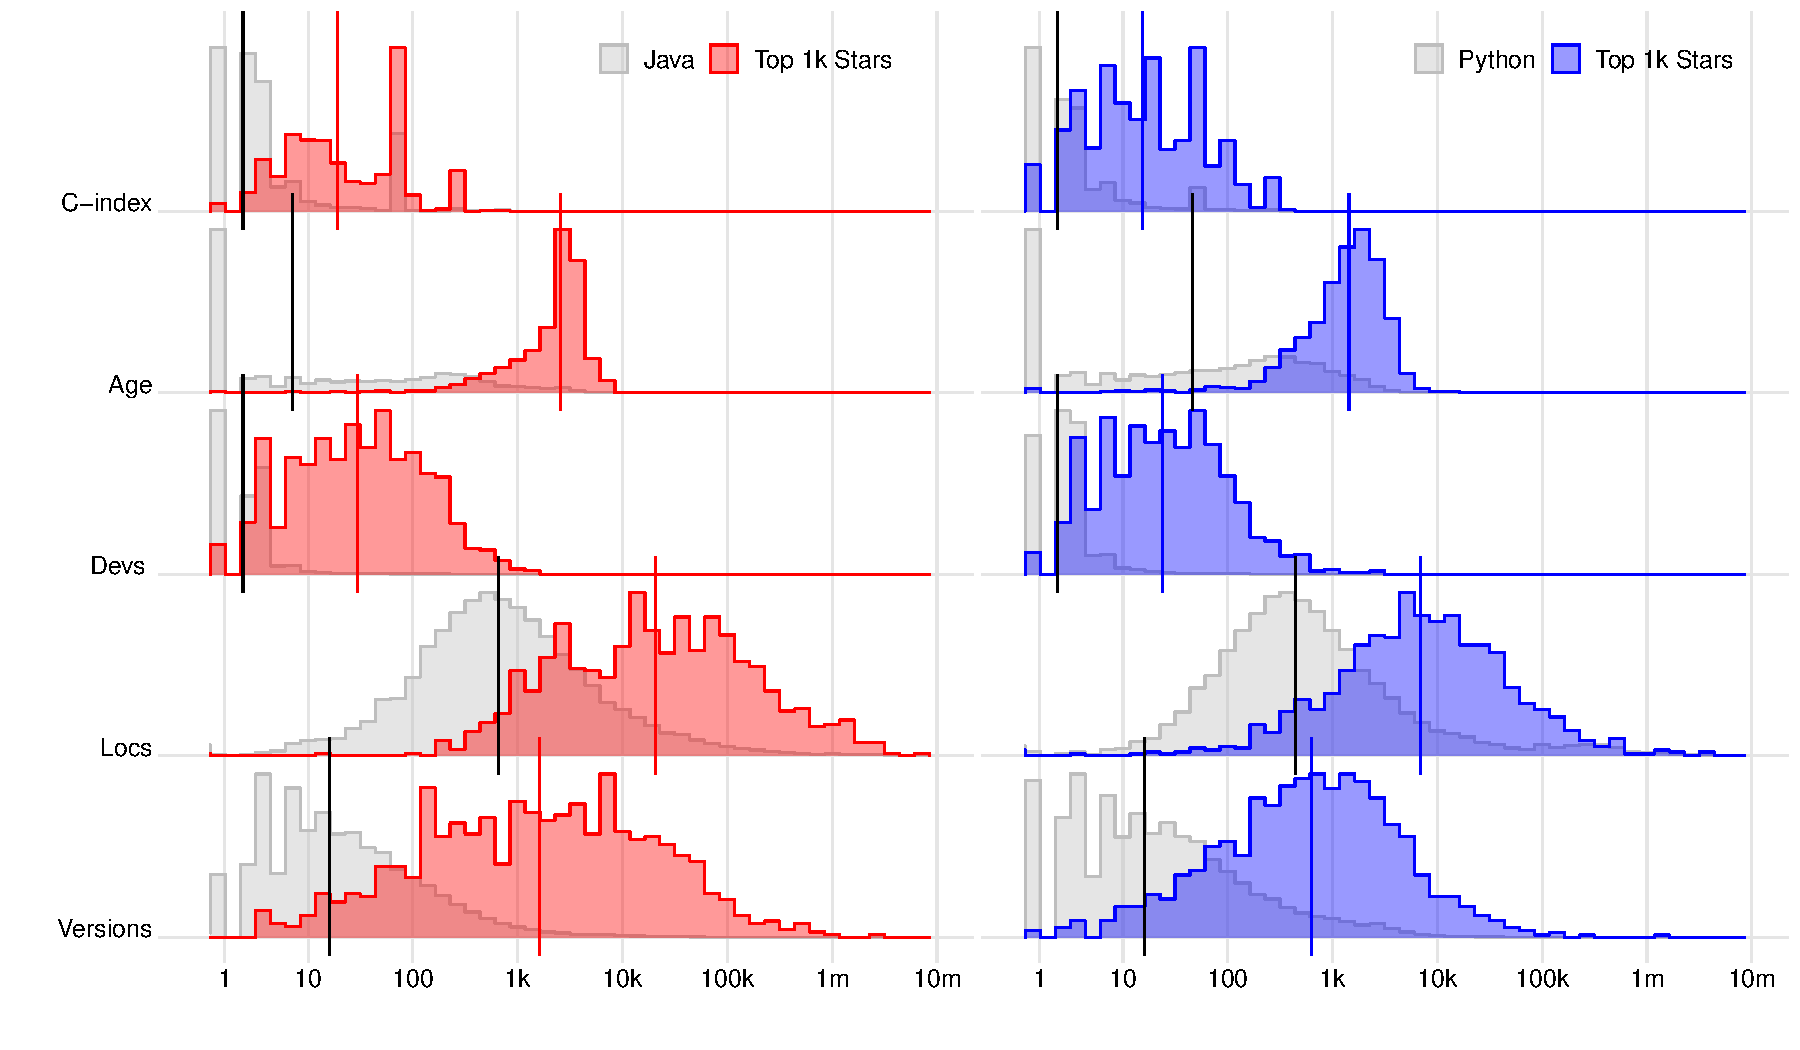
\includegraphics[width=.9\textwidth]{../figs/lang_stars_attributes}
    \caption{Comparing datasets}\label{dataset}
\end{figure*}

\section{Mapping the \gh Landscape}

The meta-study of Table~\ref{tbl:msr-summary} highlights the dominant position
of \gh as a data source in large-scale code analysis studies. We claimed that
convenience sampling using stars as a proxy for various other characteristics of
``real-world'' software is flawed. While this may sound plausible to some
readers, it should be backed up with data. Given the size of \gh, this section
uses sampling to answer the following questions: {\it Are starred projects a
  representative sample of all projects?} and {\it Are starred projects a
  representative sample of developed projects?} where what it means for a
project to be developed is purposefully left open.

Since the later parts of this paper require Java, Python and JavaScript, we
acquire samples of these three ecosystems. We use \dj to do this. \dj is an open
source project that can be forked and used to create a dedicated project
database. \dj ensures reproducibility of queries over the database and generates
reproduction receipts for all queries used in this paper.

We used random sampling over the entire \ght dataset to select which
projects to acquire in each of the languages of interest. The number of
downloaded projects is somewhat arbitrary as it is based on available hardware
during the acquisition phase which began on April 1st, 2021. The datastore has
\javaActualProjects Java projects, \pythonActualProjects Python projects and
\jsActualProjects JavaScript projects (include source code). To give an idea of
the scale, our Java dataset accounts for 20\% of all non-forked \gh Java
projects. For simplicity, we down sampled further, randomly selecting 1Mio Java
and JavaScript projects, and 200K Python projects.

\subsection{Attributes}

With \dj, it is easy to write queries that compute project attributes. For this
paper, we calculate 36 attributes for each project. From these, we select five
attributes that highlight the differences between projects:
\begin{itemize}[leftmargin=*]
\item{{\bf Age:}} The age of a project is the number of day separating the first
  commit and the most recent commit. This correlates with the maturity of a
  project.
\item{{\bf Devs:}} The count of unique developer handles in the git logs;
  includes both the author of a code change and the committer of that change.
  Devs approximates the size of a team, of course some individuals may have more
  than one handle.
\item{{\bf Locs:}} The total number of lines in files that are recognized as
  code, in any language, and appear in the head of the default branch. Locs
  measures the active code in the project.
\item{{\bf Versions:}} A version is implicitly created for each commit touching
  a file, be that for insertion, deletion or update. This counts versions in the
  entire project's history including branches. Versions measure the activity in
  a project.
\item{{\bf C-index:}} A developer handle has a c-index of $n$ if that developer
  was party to at least $n$ commits to $n$ projects (i.e. $n^2$ commits). The
  c-index of a project is the highest such number across developers. This
  measures developer expertise.
\end{itemize}

\noindent
While we make no claims that these five attributes suffice to describe a software
project, we have found them to be an effective summary of many interesting
dimensions.


\subsection{Stars v. All}

What do these attributes tell us about the overall population and about starred
projects? Fig.~\ref{dataset} is a histogram of attributes, the x-axis is log
scaled and the y-axis is normalized for maximum height. In grey (background) is
the whole population, red (Java) and blue (Python) are used for the 1K most
starred projects.

The whole population is similar across languages. Most projects are young, with
\javaLessThanWeekPct/\pyLessThanWeekPct (J/P) of projects less than a week old,
and with median ages of \javaLifetimeMedian/\pyLifetimeMedian days. Many
projects are the work of a single developer, medians are
\javaDevsMedian/\pyDevsMedian Devs. Most project are small, medians are
\javaLOCSMedian/\pyLOCSMedian Locs. Median versions are
\javaChangesMedian/\pyChangesMedian. Finally, the C-index is low, with medians
of \javaCIndexMedian/\pyCIndexMedian.

Unsurprisingly, Fig~\ref{dataset} confirms that starred project, and in
particular the top 1K, have a very different make up than the overall population
of \gh projects. Visually it is obvious that every distribution is shifted
towards older and larger projects with more developers and these being more
experienced. While there are slight differences between languages, the overall
picture is consistent. The greatest shift is in project ages with medians of
\JavaMedianOneKStarsLifetime/\PythonMedianOneKStarsLifetime days, i.e. many
years old projects. C-Indices also increase, with medians of
\JavaMedianOneKStarsCIndex/\PythonMedianOneKStarsCIndex, suggesting that active
developers tend to contribute to popular repositories. While many of them are
team efforts, a significant portion has few contributors. Manual inspection
revealed that any starred projects have been inactive for years. Project cannot
``loose'' stars, so if project gets to the top there is a chance it will stay
there long past its useful lifetime.

We can now answer the first question by the negative. Starred projects do not
yield a representative sample of the overall population. Now, this is not
necessarily a bad thing, as folklore suggests that most of \gh is uninteresting.

\subsection{Stars v. Developed}

Many researchers yearn for \emph{engineered} \cite{mun17,pick19} or
\emph{developed} projects -- informally, taken to mean projects that have been
created with some care -- alas there is little agreement on a precise
definition. Slightly easier, perhaps, is to settle on what we don't want, the
projects that are clearly of little value for any reasonable research question.
Moreover, one could hope that the complement of uninteresting projects are the
projects we want to analyze. Let us define a project that has less than
\uninterestingLocs lines of code, fewer than \uninterestingLifetime days old,
and fewer than \uninterestingCommits commits as \emph{uninteresting}. When this
definition is used to filter projects, this rather low bar manages to eliminate
\javaUninterestingProjectsPct of Java and \pythonUninterestingProjectsPct of
Python projects.

\begin{figure}[!b]
  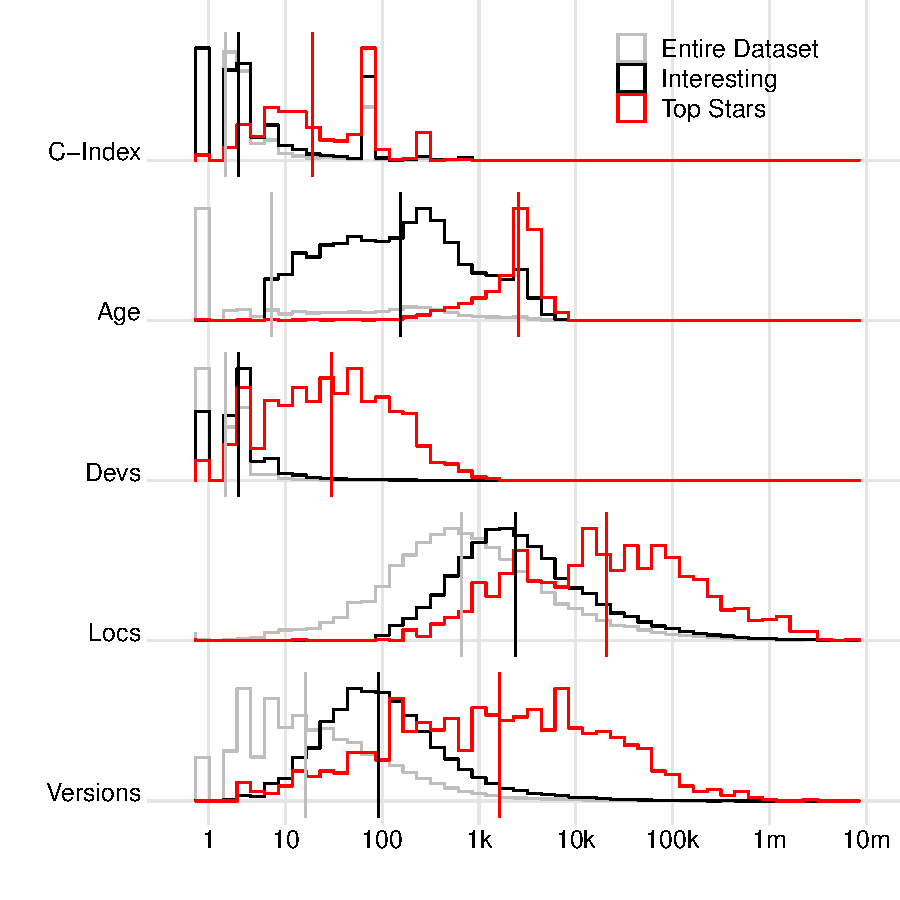
\includegraphics[width=.9\columnwidth]{../figs/lang_interesting_stars}
  \caption{Comparing developed and starred projects}\label{interestingVsStars}
\end{figure}

It would be handy if stars were a proxy for filtering out such uninteresting
projects. Fig.~\ref{interestingVsStars} overlays the whole population (grey),
the result of removing uninteresting projects (black) and the top 1K starred
projects (red for Java, blue for Python). Sadly, developed projects do not align
with stars. In terms of lines of code, developed projects have roughly the same
distribution as the whole population but biased towards larger projects. Stars
push the distribution much further. As for ages, our criteria filters out a
large number of short lived projects, but stars skew significantly older.

\newpage

Manual inspection of the starred project highlights their main issue
-- stars are extrinsic properties without a direct connection to any
attributes of a project, and unlike attributes stars grow
monotonically. Thus their meaning is unclear. Users award them for
various reasons including humor and shock value.  Some projects earned
many stars because of a joke not fit for a research
paper,\footnote{\url{https://github.com/dickrnn/dickrnn.github.io}}
another has invalid code and a documentation daring users to star
junk.\footnote{\url{https://github.com/gaopu/java}}  While these
remarks might seem off-topic, they illustrate that stars do not
correlate with quality or usefulness of repositories.

To further illustrate the limitation of stars as a filter, we take, for each
attribute, the 20 lowest scoring Java and Python top starred projects.
Table~\ref{cat} has our manual classification. Arguably none of these projects
is particularly useful: externals lack histories, widgets are small and biased
by their application domain, babies are too small to yield much insights, and
the others only have code snippets.

\begin{table}[!h]\small
\begin{tabular}{|p{6cm}|l|l|}
 \hline
 Category & Java  &Python\\\hline
 {\bf Externals} &  9\% & 5\%\\\hline
 \multicolumn{3}{|p{8cm}|}{ \footnotesize Very few commits, likely
  from another repository, occasionally synchronized.}\\\hline
  {\bf Widgets} &  43\% & 0\%\\\hline
  \multicolumn{3}{|p{8cm}|}{ \footnotesize
  Tiny projects with little activity that implement popular UI widgets or plugins.}\\\hline
  {\bf Docs} &  4\% & 15\%\\\hline
  \multicolumn{3}{|p{8cm}|}{ \footnotesize
  Interview questions, code snippets, course materials, card games, knitting
  patterns.}\\\hline
  {\bf Tutorials} &  17\% & 9\%\\\hline
  \multicolumn{3}{|p{8cm}|}{ \footnotesize
  Educational materials, tutorials and example applications.}\\\hline
  {\bf Babies} &  16\% & 32\%\\\hline
  \multicolumn{3}{|p{8cm}|}{ \footnotesize
  Valid but extremely small projects with little activity.}\\\hline
  {\bf Artifacts} &  0\% & 21\%\\\hline
  \multicolumn{3}{|p{8cm}|}{ \footnotesize
  Artifacts for (mostly ML) research papers. Likely developed elsewhere.}\\\hline
  {\bf Deprecates} &  1\% & 5\%\\\hline
  \multicolumn{3}{|p{8cm}|}{ \footnotesize
  Deprecated projects, no code on the main branch.}\\\hline
\end{tabular}
\caption{Categorizing 200 starred projects}\label{cat}
\end{table}

Fig.~\ref{cat} answers our second question, developed projects are broadly
similar in terms of distribution of attribute values as the whole population.
For all attributes starred projects trend towards higher values. To summarize
what we learned about stars, they capture extrinsic characteristics of \gh
projects and are at best indirect and noisy proxies for a robust frame oracle.

\subsection{How to select projects?}

What to use for project selection if not stars? We argue that selection must be
based on intrinsic features -- measurable attributes of a project's contents or
origin. While one may use machine learning~\cite{mun17,pick19} to build
classifiers, we propose to leverage the discriminative power of our five
attributes as a frame oracle.

\begin{figure}[!t]
 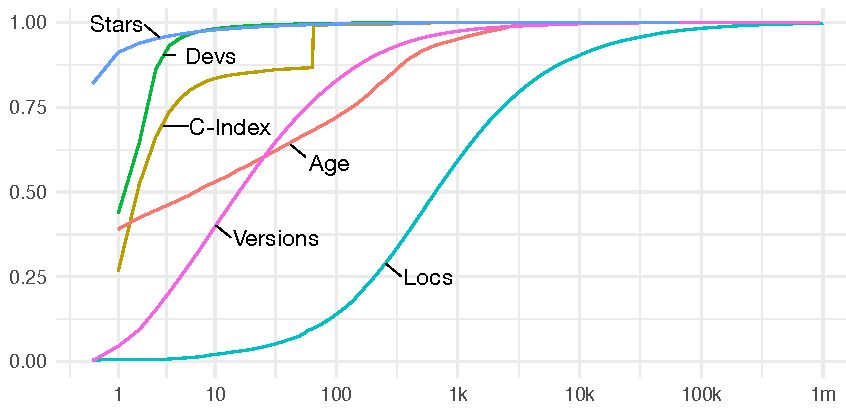
\includegraphics[width=\columnwidth]{../figs/lang_cdf_annotated}
  \caption{Cumulative Density Functions}\label{cdf}
\end{figure}

Fig.~\ref{cdf} is the cumulative density function of the various attributes for
Java (Python is similar). The interpretation of each line is what percentage of
the dataset is filtered for a particular attribute value. So for instance, if
one were to use 10 days as a cutoff, then \javaLessThanTenDaysPct of the Java
set would be filtered out. Half of Java projects have been around for less than
10 days! What also stands out is that \javaNoStarsPct of projects do not have
any stars. A 10 star cutoff one filters out \javaLessThanTenStarsPct of all
projects. The discontinuity of C-Index at 65 is worrisome. After investigation,
we found a single \gh 'developer' with such a high index, it turns out that it
is a bot doing automated updates.

Project selection can be performed by a combination of attributes with cutoffs.
We do not argue for a particular formula; researchers must make their own choices
in this respect.

\subsection{Validity}

Working with the dataset, we noticed an oddity around project ages. Experience
with \gh trained us to expect the unexpected. Our investigation started with a
plot of creation dates. Fig.~\ref{createdTime} shows the log scaled counts of
new projects over time. While there is a steady progression in the count of
projects created each year, we see a significant drop in 2015 and a plateau
until 2019. We reviewed our pipeline to no avail. We use \ght to acquire all
available URLs. Then, we randomly sample projects from that list. We validated
both acquisition and sampling. This leaves with two hypotheses. First is a
consistent flaw in the \dj downloader causing some projects to fail to download.
\jsProjectErrorsPct URLs obtained from \ght point to dead projects, but there is no apparent
bias. Second some projects could be missing in \ght. Again, we have not been
able to eliminate this possibility. Another issue showed up on inspection,
JavaScript project ages are significantly higher than those of other languages.
We found that \gh timestamps are frequently inconsistent, but why JavaScript be
more affected? Until an explanation can be found, we removed JavaScript from the
overall comparison and use JavaScript projects in the reproduction with extreme
care.

\begin{figure}[!h]
    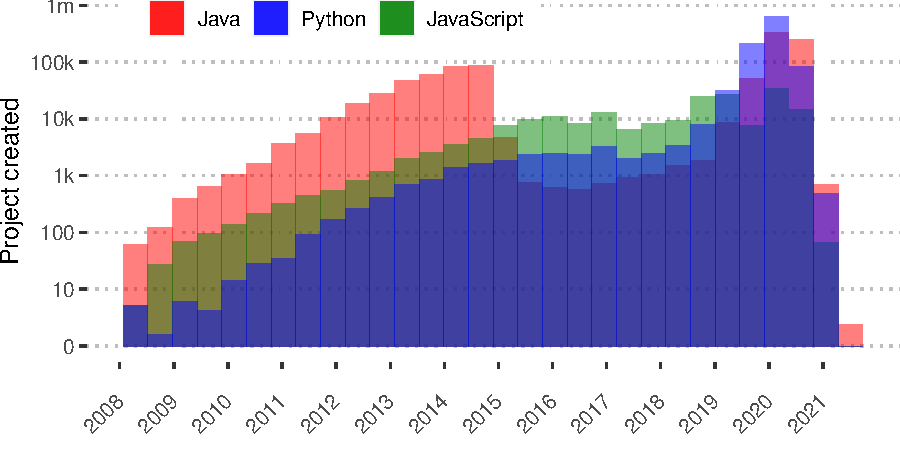
\includegraphics[width=\columnwidth]{../figs/lang_projects_created}
    \caption{Creation date }\label{createdTime}
\end{figure}

\section{Reproducible Experiment Design}

This paper proposes that researchers conducting experiments over large-scale
software repositories follow a specific experimental design methodology to
ensure their work can be reproduced and increase chances their results
generalize as expected. While the mechanics of reproducibility of the actual
experiment itself vary, the setup of the experiment is a common problem. The
proposed methodology has five steps, we encourage researchers to document each
of these steps explicitly.

\subsection{Population Hypothesis}

Formulating a population hypothesis lets researchers stake a claim about the
applicability of their work. This represent the population to which the result
of an experiment should generalize to. The statement of that hypothesis can be
brief and appeal to intuition, the other parts of the description flesh out
the details.
%
Ideally we would like our results to be as broadly applicable as possible, but
pragmatically designing experiments that back up overly broad claims is
difficult. Some populations of interest are difficult to sample, for instance
``commercial software'' is a relatively simple and unambiguous description but
one that we typically can't sample from as most of the software is not in the
public domain. Other populations can be difficult to identify. Imagine a study
of the challenges linked to retraining imperative programmers to use functional
idioms. Finding code written by such developers can be done manually but is
difficult to automate. It is often easier to describe a population by intrinsic
features of projects such as the language used to write the code or some
estimate of the size of the project.

\subsection{Frame Oracle}

A frame oracle is a, possibly noisy, deterministic algorithm for deciding if a
project belongs to the population of interest. The oracle is our best
approximation of the population of interest. An executable and reproducible
oracle allows to compare different papers with the same selection. The
description of the oracle should specify the data source along with any
information required to acquire projects. The procedure for evaluating a project
should be clear and based on intrinsic attributes. A paper should at least have
a short description of the oracle, full details should be given in the
reproduction artifact.

\subsection{Sampling Strategy}

The literature has an abundant advice on sampling (see e.g.
\cite{Lohr:2010:Sampling}). Briefly, a sampling strategy picks the type of
sampling (probabilistic or non-probabilistic) and describe the high-level steps
used to obtain a sample. The sampling implementation is expected to be found in
the reproduction artifact. Many works use purposive or convenience sampling as
it is simpler, cheaper and less time consuming. A better alternative is some
form of probabilistic sampling as it is more likely to yield a representative
sample. Probabilistic sampling can be staged if the structure of the population
is more complex. The simplest approach is random sampling where each element has
the same chance of being picked. We often have to resort to stratified sampling
when the population is divided in subgroups of different sizes. Typically we
sample without replacement as we do not want to pick the same project multiple
times.

\subsection{Validity}

The validity section should argue, when there are reasons for doubt, why using
the frame oracle and the sample strategy results in representative samples of
the population. This section should also address potential sources of bias and
attempts by the authors to control for them. This section should address any
foreseen challenges to reproducibility and offer means to mitigate them.

\subsection{Reproducibility Artifacts}

The last components of our approach is to link the paper to a reproduction
artifact that contains code and data to support experimental repeatability and
reanalysis.

\subsection{Tool support}

Section 3 has listed specific issues with reproducibility. Roughly, there are
two kinds of issues. The first is related to authors not being precise in their
description of some of the steps outlined above. We believe that following the
methodology as a template in the text of a paper and providing a reproduction
artifact will greatly help. The second category of issues are more pragmatic, it
is difficult to repeat the analysis of a paper because some aspect of the data
used is not available. We suggest that research infrastructures should support
the task by explicitly supporting experimental reproducibility. An example of
such an infrastructure is \dj which is both a continuously updated datastore and
a database that can be queried by a DSL written in Rust. We have adopted that
infrastructure for our work and illustrate how it helps with reproducibility.

The implementation of a frame oracle and the sampling strategy can be combined
into a single expression. Fig.~\ref{fig:style-analyzer-query} shows a query
which starts by filtering out projects with fewer than 80\% JavaScript code,
then it uses pre-computed attributes Locs, Age and Devs to filter further. The
last stage of filtering involves computing an attribute on the fly, here we sum
up the commits in the project. Random sampling is implemented by calling the
\c{sample} function.

\begin{figure}[!h]
  {\footnotesize\begin{verbatim}
database.projects()
  .filter(|project| {
      project.language_composition().map_or(false, |languages| {
          languages.into_iter().any(|(language, proportion)| {
              language == Language::JavaScript && proportion >= 80
          })
      })
  })
  .filter_by(AtLeast(Locs, 5000))
  .filter_by(AtLeast(Age, Duration::from_months(12)))
  .filter_by(AtLeast(Devs, 2))
  .filter_by(AtLeast(Count(Commits), 100))
  .sample(Random(30, SEED)))
\end{verbatim}}
\vspace{-4mm} \caption{Project selection with \dj}\label{fig:style-analyzer-query}
\end{figure}

The architecture of \dj is split between a persistent datastore in which every
data item is timestamped with an insertion data, and an ephemeral database used
to service queries. A reproducible query is a Rust crate archived in a git
repository associated to the datastore. Running the query produces a
\emph{receipt} which is the hash of a commit automatically added to the archive
repository. The receipt can be used to share the query (exactly as executed) and
its results (exactly as produced). It can be used to retrieve the Rust crate and
re-execute the code. Code re-execution is helped by the fact that queries are
deterministic and the crate contains a list of all dependencies, a timestamp,
and all random seeds. When a historical query is executed \dj access the exact
state of the datastore at the time the query was run. Since \dj stores the
contents of files, entire experiments can be fully reproduced.

\newpage

\section{Reproductions}

We demonstrate the value of the methodology with examples. Results suggest that
additional experiments are needed to validate some of the claims made in the
reproduced works.

\subsection{Reproducing: What is Software}

This reproduction aims to validate two simple findings of \citet{Pfeiffer20}:
(C1) sowftare is diverse, only 4\% of repositories do not contain code, data and
documentation; (2) documentation is an integral constituent of software, only
2\% of repositories do not contain documentation. Our methodology is to start by
a reproduction that attempts to follow the paper. Then we investigate if the
results generalize to the intended population.

\P{Population Hypothesis:} The entire universe of software projects.

\P{Frame Oracle:} To understand the impact of project selection we consider
three oracles. O1 accepts any software project hosted on \gh. O2 is subset of O1
with uninteresting projects removed (as defined above). O3 uses a stronger
filter, removing projects with fewer than 500 commits, 180 days, or 10K Locs. We
use \gh language attribution to select a project's language.

\P{Sampling Strategy:} We report on four samples. S0 is a convenience sample of
starred projects from O1 following \cite{Pfeiffer20}. S1, S2 and S3 are random samples
without replacement from O1, O2 and O3 respectively, stratified by language.
Projects with duplicate contents are removed.

\P{Validity:} Our reproduction differs in the number of languages (3 v. 25) and
by categorizing files based on the file path alone. We tested stability of our
results with multiple samples of varying sizes and manually inspected the produced
labels.

\P{Reproduction Artifact:} Our artifact has \dj receipt for this query.

\vspace{-5mm}

\begin{figure}[!h]
   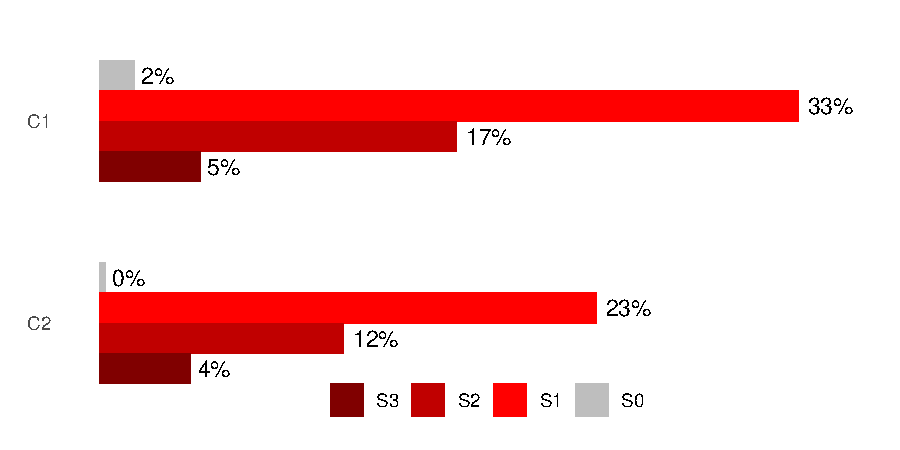
\includegraphics[width=\columnwidth]{../figs/what-constitutes-software/software.pdf}
\caption{Content of software projects}\label{sw}
\end{figure}

\vspace{-5mm}

\subsection*{Results}

Fig.~\ref{sw} shows the results of reproduction for claims C1 and C2. Compare
the percentages between S0 (original) and S1 (target population). Statistical
analysis is not required to see that the difference is significant. The samples
S2 and S3 are there to illustrate the impact of slightly more developed
populations, but even these are still quite different. Would the results agree
if we included more languages? The three languages we downloaded account for
most of \gh, it is conceivable that other languages could affect results, but
that would just push the generalizability issue somewhere else as the claims would
become language-specific.

\newpage
\subsection{Reproduction: Method Chaining}

\citet{nakamaru:2020:MSR} claim that 50\% of projects in 2018 had method chains
longer than 7 while in 2010 that number was 42\%, and more generally they
observed longer chains at all lengths. They state that ``chains of length 8 are
unlikely to be composed by programmers who tend to avoid method chaining, this
result is another supportive evidence for the widespread use of method
chaining.'

We intend to reproduce the authors methodology, and then compare to various
samples that might represent that the authors expresed as their population of
interest in their paper.

\P{Population Hypothesis:} The universe of real-world Java programs.

\P{Frame Oracle:} We accept any Java project hosted on \gh
and delegate to GitHub for language attribution.

\P{Sampling Strategy:} Stratified sampling to randomly select projects with commits
in 2010 and 2018.

\P{Validity:} To reproduce the original results, we performed stratified
sampling to get top starred projects active in the target years. The authors
used a different sample of top stars. The original paper had different sample
sizes for each year, but those are not specified. We fix the sample size to 250.
The authors could not locate the code of their chain detector, so we use
our own implementation.

\P{Reproduction Artifact:} The selection of input is represented by a \dj
receipt in the artifact.

\begin{figure}[!h]
  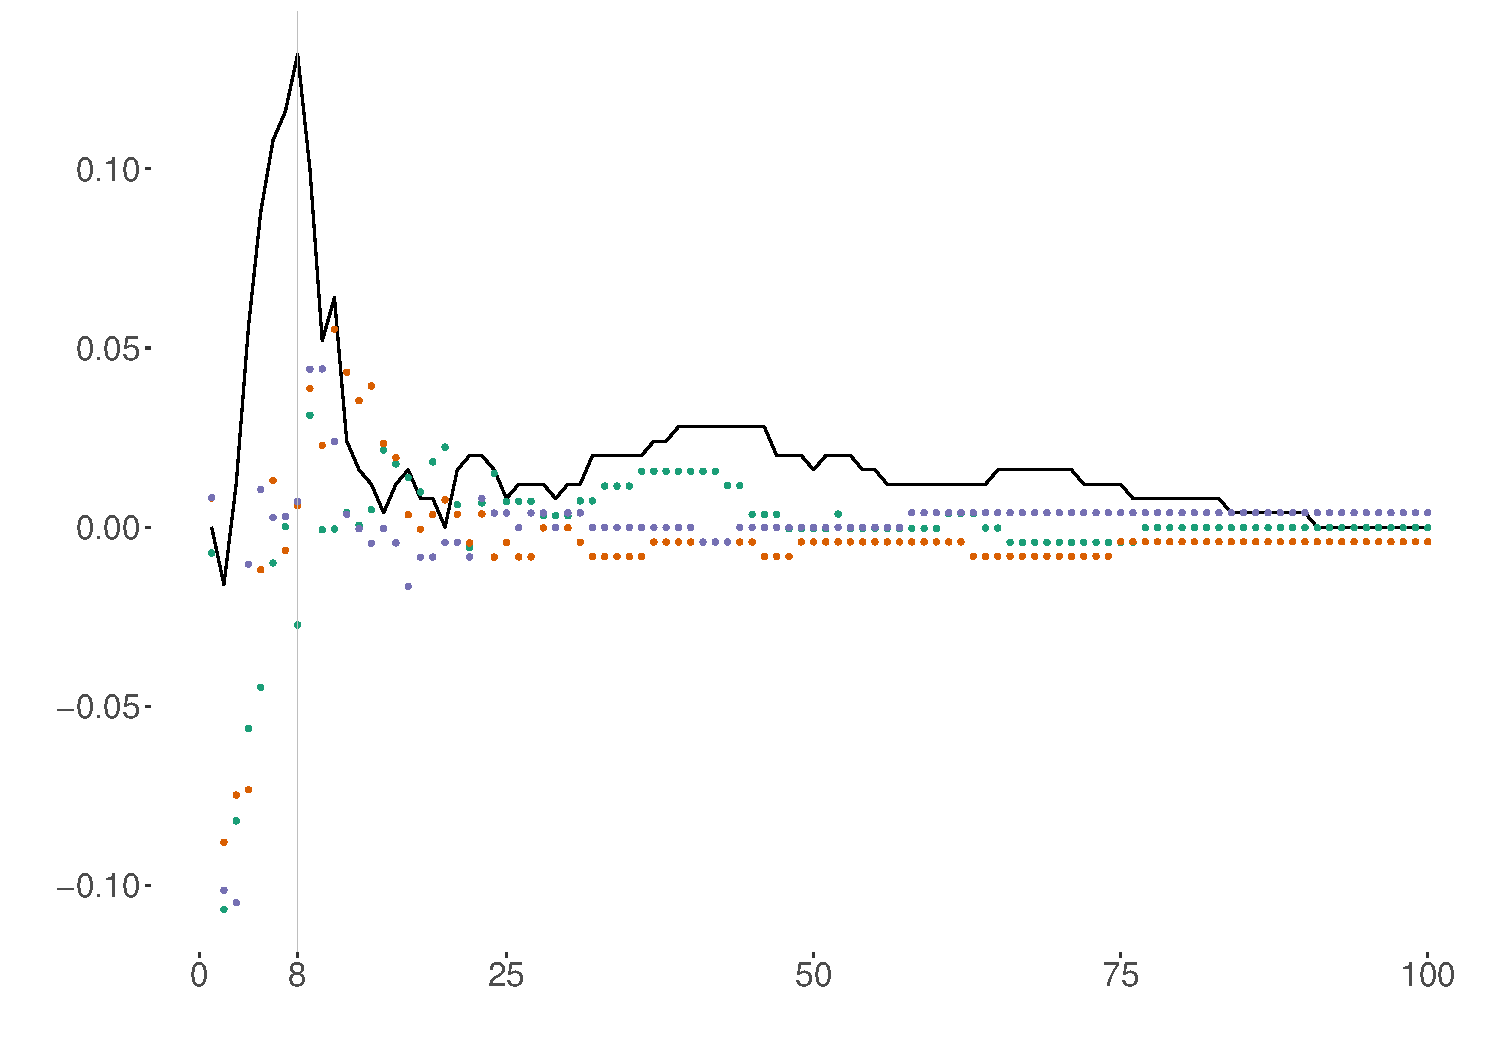
\includegraphics[width=\columnwidth]{../figs/method_chainings/final_graph.pdf}
  \caption{Difference in chain lengths}\label{fig:un_difference}
\end{figure}

\subsection*{Results}

Fig.~\ref{fig:un_difference} shows the difference in proportion of projects at
various chain lengths. The solid line uses stars, colors represent different
random samples. For instance, if we pick chains of length 8, the number used by
\citet{nakamaru:2020:MSR}, the difference is a 13\% increase in the number of
projects between 2011 and 2018. The differences for our random samples are -2\%,
0.6\% and 0.7\%. This particular population does not seem to show the effect
expected by the authors. We surmise that some notion of developed project may
show more favorable results, but without more guidance in the population
hypothesis it is hard to guess which to pick.


\newpage
\subsection{Reproduction: Style Analyzer}

\citet{Markovtsev:2019:MSR} build model of the style of a repository and apply
this model on a held-out part of that repository to produce corrections. Their
experiment uses 19 top-starred JavaScript project to gauge the precision with
which the tool flags formatting discrepancies and the relationship between this
precision and the size of the project. They report a precision of 94\% (average,
weighed by project size) and better overall performance for large projects and
projects with better style guidelines.

We investigate how different project samples impact these conclusions. For the
reproduction we attempted to create samples to fulfill our intuition about the
original's paper intentions as best we understand them from the conclusions they
draw.

\P{Population Hypothesis:} A developed JavaScript projects.

\P{Frame Oracle:} Our oracle picks JavaScript projects such they contain at 80\%
JavaScript code (files), Loc $\geq 5000$, Age $\geq 12*31$ and Devs $\geq 2$.

\P{Sampling Strategy:} We randomly select 10 sets of 30 projects. We select more
projects than the original sample to account for errors in processing. After
processing is finished, we randomly select 19 out of the pool of successfully
processed projects in each selection.

\P{Validity:} Given the complexity of the tools configuration and the fact that
it is missing from the artifact, we used a default configuration provided by the
tool. This produces an average increase in project size by
\SAMeanSupportDeltaPaperVOriginal per project (up to a maximum of
\SAMaxSupportDeltaPaperVOriginal) and causes precision to diverge by
\SAMeanPrecisionDeltaPaperVOriginal on average, and up to
\SAMaxPrecisionDeltaPaperVOriginal.

The tool failed to process 4 projects: \texttt{freecodecamp} and \texttt{atom}
due to errors in unicode processing, \texttt{express} due to a programming bug,
and \texttt{30-seconds-of-code} probably due to bad file identification. Three
of the missing projects were located close to the median in terms of precision,
prediction rate, and project size in the original paper, while \texttt{axios}
was in the lower quartile for sample count. We reproduced the study using
19-project samples.


Style analyzer analyzes each project at two points in its history specified by a
base commit and a head commit. The base commit is a point in the past which the
tool checks out to learns the project's formatting style. The head commit is a
more recent point used to evaluate the model and calculate precision. The
original paper provides head and base commits for each project in their
experiment, but does not specify the method of selecting these commits. We pick
the current head of the default branch as the head commit. For base commit we
pick one that lies at an offset equal to 10\% of the number of all commits in
the default branch from the head commit. This retrieves different commits than
the original paper, which causes a \SAMeanPrecisionDeltaOriginalVRepro median
change in precision (up to
\SAMaxPrecisionDeltaOriginalVRepro---\texttt{telescope}) and a median project
size increase of \SAMeanSupportDeltaOriginalVRepro, and up to
\SAMaxSupportDeltaOriginalVRepro (\texttt{reveal.js}).

\P{Reproduction Artifact:} Datasets, receipts from submitted \djco queries,
style analyzer's reports and scripts for the entire experimental pipeline are
included in the artifact.

% Errors: local variable 'next_vnode' referenced before assignment <- don't use
% dynamic languages, kids
%
% ValueError: Found array with 0 sample(s) (shape=(0, 4185)) while a minimum of
% 1 is required <- not sure why, my **guess**, is it has something to do with
% the fact that the JS code is not in .js files, and the tool can't handle that.
%
% KeyError: 6663 <- this unicode related
%
% KeyError: 138726 <- this is unicode related

% Since the selection used by the original paper was small, we decided to
% reproduce the experiment by selecting multiple additrional samples of
% top-starred JavaScript projects. We produced 10 selections of 30 projects each
% by creating an oracle frame of 300 top-starred JavaScript projects and splitting
% the entire frame into 10 separate samples. We select more projects than the
% original sample to account for errors in processing. After processing is
% finished, we randomly select 19 out of the pool of succesfully processed
% projects.

\begin{figure}[th]
  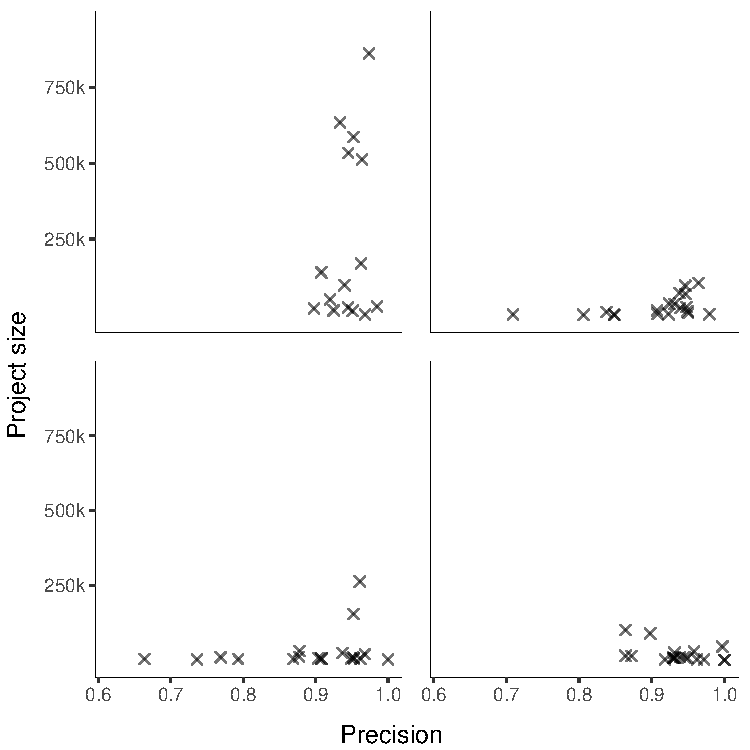
\includegraphics[width=.8\columnwidth]{../figs/style-analyzer/precision-vs-samples.pdf}
  \caption{Relationship between label groups and precision}\label{fig:precision-vs-samples}
\end{figure}

\begin{figure}[th]
  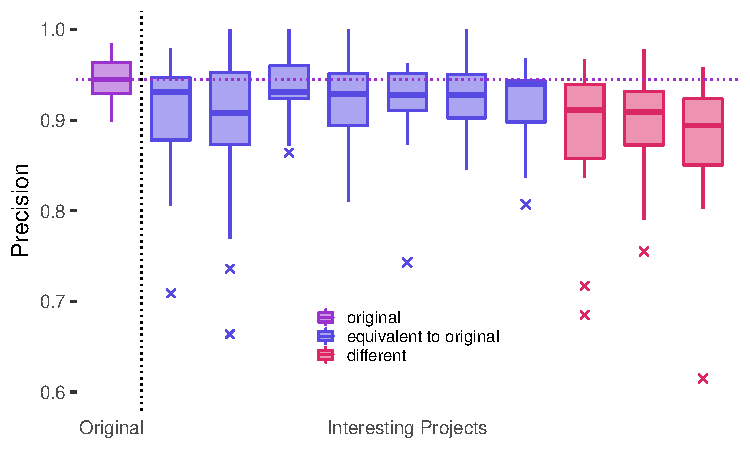
\includegraphics[width=\columnwidth]{../figs/style-analyzer/precision-and-samples-comparison.pdf}
  \caption{Comparing label group count and precision}\label{fig:precision-and-samples-comparison}
\end{figure}


\subsection*{Results}

We recreate a plot of the effect of the number of items in the training set on
precision from the original paper in Fig.~\ref{fig:precision-vs-samples}. The
training set consists of snippets created around tokens/AST nodes relevant to
formatting (whitespace, indentation, quotes, zero-length gaps). We plot the
selection from the original paper along three selections from our interesting
project frames.
In addition, we plot the distributions of precision in each selection in
Fig.~\ref{fig:precision-and-samples-comparison}. We compare the precision scores
in each sample with the selection used in the original paper using a
Mann-Whitney U test to show which samples performed statistically differently
from the original. % (using a p-value of $0.05$).
The scatter plots show a different grouping of results from the original paper.
The groupings in the scatter plot visibly differ between selections. The
distribution comparison shows that our selections generate significantly smaller
training sets in all cases and yield lower precision. In addition,
\SADifferentSelections out of the \SAAllSelections interesting project
selections produced significantly lower precision, with the remainder producing
a statistically equivalent distribution.

Overall, we see our selections yielding
precision between \SAMinPrecision and \SAMaxPrecision (the paper sets
a precision of 0.95 as a benchmark for success). We also do not see a clear
relationship between the number of label groups and precision, such as the one
the authors note in the original paper.

\newpage

\subsection{Reproduction: Code Smells}

We seek to validate the claim of \citet{Jebnoun:2020:MSR} that for large and
small projects there is a statistical difference in the occurrence of code
smells, whereas medium sized projects are indistinguishable.

\P{Population Hypothesis:} Mature \gh projects in all application domains
including machine learning written in Python.

\P{Frame Oracle:} Projects with C-Index $\geq \dlHIndexLowerboundOr$, or Age
$\geq \dlLifetimeLowerboundOr$, or Locs $\geq \dlLocsLowerboundOr$, or Versions
$\geq \dlCommitsLowerboundAnd$. We delegate to \gh for language attribution.

%%% TODO:: SWITCH TO Use versions in the repro

\P{Sampling Strategy:} The deep learning projects were provided by the authors.
Out of 59 projects, 57 were still accessible on August 2nd 2021. At download
time there were \countSmallDL small, \countMediumDL medium, and \countLargeDL
large deep learning projects. For the reproduction of the original results, we
used a staged strategy, first convenience sampling the top starred Python
projects and amongst those used stratified sampling to select 57 projects with a
similar distribution of sizes. To generalize the results we used quota sampling
to match the size distribution.

\P{Validity:} Our reproduction uses the Locs reported by \dj. The date the
authors downloaded the repositories is unknown. We use the content of the main
branch of each repository as of April 1st, 2020. The authors say ``\textit{each
  of repositories is pre-processed and prepared for code smell detection}'',
however details are missing. We used the default thresholds of their tool.

\P{Reproduction Artifact:} A \dj receipt is included in our reproduction package
along with code to run the experiment.

\begin{figure}[th]
  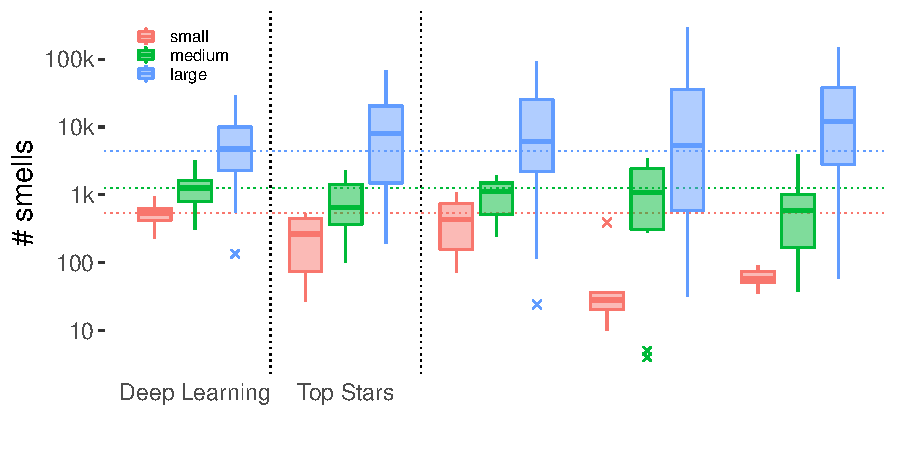
\includegraphics[width=1.03\columnwidth]{../figs/scent-dl/smell_frequencies}
  \caption{Comparing Smells}\label{fig:smell_frequencies}
\end{figure}


\subsection*{Results}

Fig.~\ref{fig:smell_frequencies} contrasts the distribution of smell for deep
learning projects, top stars, and three random samples. Computing the p-values
with the non-parametric Mann-Whitney Wilcoxon shows that one of the samples
disagrees on small projects (i.e. the difference is not statistically
significant) and two of the samples disagree on the large projects (again the
difference is not significant). Generalizability of the results is thus
questionable.

\section{Conclusions}

Sometimes doing it wrong is so much easier than the alternative, that we
convince ourselves that the wrong is right enough.

Our paper is unusual. While it purports to contain a call to arms for better
experimental practices, it is just as much a record of our own journey to that
goal. What reads as criticism was just as likely written in self-reflection. So,
what can a researcher in the field take away from this paper? There are three
ideas we would like to leave you with regarding \emph{generalizability},
\emph{reproducibility} and \emph{tooling}.

\paragraph{Generalizability.} The value of an experiment often lies as much
in what it generalizes to, as in the experiment's outcome. We found that many
researchers rely on \gh stars to pick representative samples of software
projects, yet starred projects tend to be larger in most dimensions than typical
ones, also that they are more likely to be inactive, and that their ranking is
not a measure of intrinsic qualities of the code. Hopefully, this paper is the
last nail in that coffin. More generally, we advocate for the use of
probabilistic sampling over populations defined by intrinsic attributes of
software, and also for clear and standardized documentation of experimental
design.

\paragraph{Reproducibility.}
The value of a scientific experiment also lies in our ability to reproduce it.
Carrying out reproducible experiments over large-scale software repositories is
hard. Especially when aiming to support the three reproduction modalities:
repetition, as practiced in artifact evaluation, where an artifact is
re-executed to obtain identical results; reanalysis, where the artifact or its
input are modified; and independent reproduction, where the entire experiment is
re-implemented from scratch. The first modality requires faithful replay and is
best served if all data used is included with the artifact. The second, requires
support for automatically acquiring new representative samples. The third needs
an unambiguous description of all experimental steps. We advocate for
reproductions artifacts that supports the first two modes, and a detailed
description of the experiment for the last.

\paragraph{Tooling.}
Generalizability and reproducibility, while worthy goals, represent much work,
and they are work that is orthogonal to the scientific goals of researchers. The
only reasonable answer is to provide tooling that automates acquisition of
representative samples and generation of reproduction artifacts. In this paper,
we used \dj and found it helpful as it let us specify queries over attributes of
the code for many projects, while also supporting experimental repetition and
reanalysis through historical queries. It has its limitations, we found
execution times to be somewhat long and doubt it will scale to the whole of \gh.

\medskip

Our vision for a bright and shiny future is one where the community agrees on
standard tools and techniques for this kind of experiment, tools which automate
the acquisition and packaging of input datasets and the re-execution of entire
experiments.

\bibliographystyle{ACM-Reference-Format} \bibliography{bib/all}
\end{document}
\endinput
